\section{Experimentos a realizar}


\subsection{Resultados obtenidos}
\noindent A continuación se presentan los archivos de salida resultantes posterior a un caso de prueba.
\begin{figure}[H]
	\centering
	\includegraphics[scale=0.5]{images/compilacion.png}
	\caption{Ejemplo Salida al compilar el codigo.}
	\label{fig:ej1}
\end{figure}

\begin{figure}[H]
	\centering
	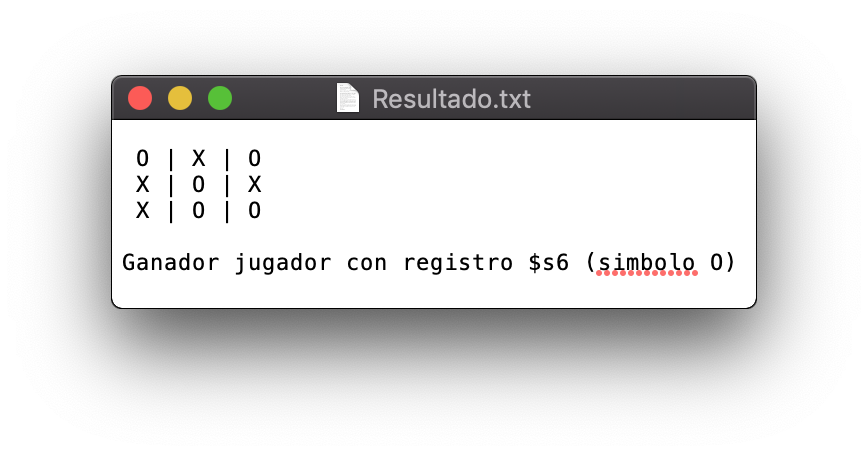
\includegraphics[scale=0.5]{images/resultado.png}
	\caption{Ejemplo de Salida del resultado del juego.}
	\label{fig:ej2}
\end{figure}

\begin{figure}[H]
	\centering
	\includegraphics[scale=0.5]{images/Etapas.png}
	\caption{Archivo de salida del camino de datos.}
	\label{fig:ej3}
\end{figure}


\subsection{Análisis de resultados}

\noindent Se ha logrado que el programa sea capaz de leer las instrucciones y las líneas de control que se presentan en un archivo de texto plano, distinguiendo en este los comentarios y valores inválidos dentro de una jugada, para luego simular su ejecución completando el tablero de manera óptima, en caso que las instrucciones se encuentren insertadas de manera correcta. El programa logra identificar de manera adecuada cuando una jugada corresponde a la victoria de un jugador en particular, un empate o un error de instrucción, el cuál entrega un mensaje de "incompleto".
